%%% intro on CERN and LHC 
%%% goals of particle physics research at CERN

\chapter{The CERN accelerator complex and the LHC}\label{chap:CERN_LHC}

The theory that currently best describes the fundamental particles and their interactions is known as the Standard Model \cite{Herrero1999}. It was developed during the 20th century and finalized in the mid-1970s, after experimenal confirmations of quarks. The Standard Model has since predicted and explained a wide range of phenomena with great accuracy, important examples are the W and Z bosons and the Higgs boson. However, some questions still remain unanswered.

\begin{figure}[!ht]
    \centering
    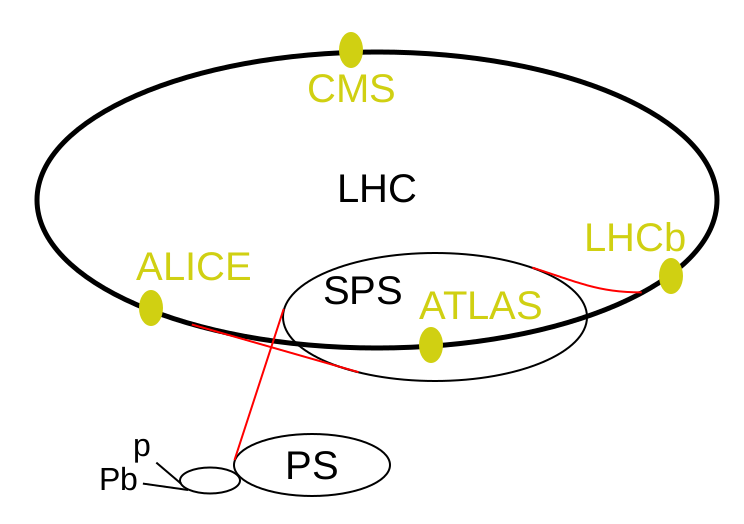
\includegraphics[width=.7\linewidth]{Images/intro/LHC.png}
    \captionsetup{width=.7\linewidth}
    \caption{Simplified scheme of the CERN accelerator complex. Each proton or lead ion starts from a linear accelerator (LINAC 4 and LINAC 3, respectively, not in the picture), it is then transferred to the Proton Synchrotron (SP), into the Super Proton Synchrotron (SPS) and finally into the Large Hadron Collider (LHC). During each phase of acceleration the particles reach higher momentum before being transferred to the next stage.}
    \label{fig:LHC}
\end{figure}

\marginpar{\flushleft I could add some details of the process of acceleration, from H atoms to proton beam into the LHC}

The Large Hadron Collider (LHC) is the largest particle accelerator in the world. It was built between 1998 and 2008 by the European Organization for Nuclear Research (CERN, \textit{Conseil européen pour la Recherche nucléaire}) in collaboration with more than 100 countries with the purpose of colliding hadrons\footnote{\label{footnote:hadrons}Hadrons are particles that are made up of two or more quarks, e.g. protons and neutrons} at high energies and study the products of these collisions. It consists of a \qty{27}{\kilo\meter} ring at roughly \qty{100}{\meter} of depth situated at the Franco-Swiss border, near Genève. Two beams of particles travel at near light speed in opposite directions inside two pipes surrounded by superconducting magnets. At specific locations the beams converge and collisions take place, these events can then be observed with specialized detectors built along the tracks.


\section{The research goals}\label{sec:CERN_research_goals}

The construction of the LHC was motivated by the need for experimental data to study the laws of our universe. In particular, its main research goals were \cite{homeFactsFigures}:
\begin{itemize}
    \item The search for the Higgs boson, the particle (whose mass could not be predicted) responsible for the origin of mass, culminated in the discovery of the Higgs boson in 2012 \cite{20121}. 
    \item Supersymmetry, a theory that hypothesizes the existence of massive partners of the particles in the current Standard Model.
    \item Dark matter and dark energy, the matter that we know only makes up a small fraction, \~4\%, of the content of the universe, and the particles or phenomena responsible for the remaining 23\% (dark matter) and 73\% (dark energy) are still unknown.
    \item Matter-antimatter asymmetry, matter and antimatter should have been produced in identical amounts during the Big Bang, but so far we have observed almost exclusively normal matter.
    \item Quark-gluon plasma, the state of matter before ordinary matter could emerge in the early stages of the Universe.
\end{itemize}

The LHC is part of the CERN accelerator complex, a chain of machines in which each link accelerates a beam of particles (protons or heavy ions) to higher energies and feeds it to the next one. A simplified version of the complex is shown in Figure \ref{fig:LHC}. The LHC began operations in 2010 with energies of \qty{3.5}{\tera\electronvolt}, increased up to \qty{4}{\tera\electronvolt} in 2012. After two years of Long Shutdown for upgrades and maintenance, activities resumed in 2015 with Run 2, when beam energies of \qty{6.5}{\tera\electronvolt} ($\sqrt{s}=\qty{13}{\tera\electronvolt}$, center of mass energy) were achieved.


\section{The main experiments}

Along the accelerator tracks there are four main experiments (Figure \ref{fig:LHC}):
\begin{itemize}
    \item ALICE (A Large Ion Collider Experiment), dedicated to heavy-ion physics\cite{homeALICE}.
    \item ATLAS (A Toroidal LHC Apparatus), one of the two general-purpose detectors, able to investigate a wide range of physics.
    \item CMS (Compact Muon Solenoid), the second general purpose detector of LHC.
    \item LHCb (Large Hadron Collider beauty), an asymmetric detector that observes mainly forward particles to study the "b quark".
\end{itemize}

Additionally, there are several other experiments part of the CERN complex, including test beam facilities in the North Area which use a particle beam from SPS to perform a variety of tests.

\begin{figure}[!ht]
    \centering
    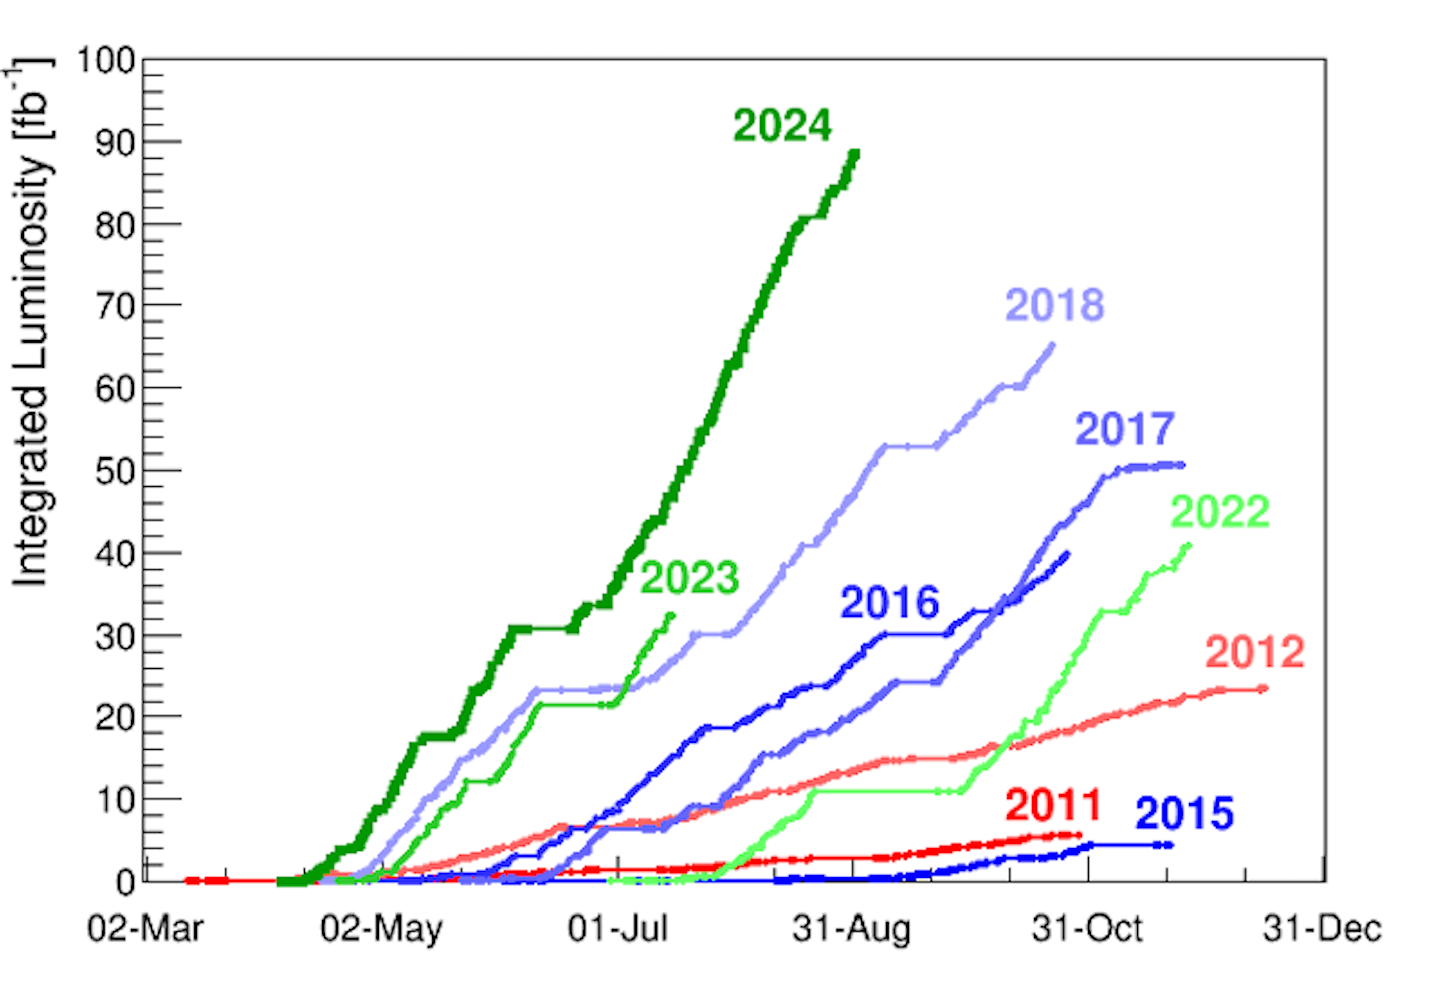
\includegraphics[width=.6\linewidth]{Images/intro/integrated_luminosity.png}
    \captionsetup{width=.8\linewidth}
    \caption{Overview of the integrated luminosity as a function of the date for each year of LHC running, with 2024 greatly exceeding all other years. From \cite{homeAcceleratorReport}.}
    \label{fig:integrated_luminosity}
\end{figure}

One of the most important parameters of a collider is the luminosity:
\begin{equation}
    L = \frac{1}{\sigma}\frac{dN}{dt} \, \left[\unit{cm^{-2}.s^{-1}}\right] \, .
\end{equation}

Where $dN$ are the number of events, $dt$ is the time interval and $\sigma$ is the cross-section: a measure of the probability that some interaction occurs. A related quantity is the integrated luminosity, which is the integral over time which quantifies that amount of data that is available to be studied, typically measured in inverse femtobarns \unit{\femto\barn^{-1}}=\qty{e-28}{\meter^{-2}}.

After the second Long Shutdown that took place between 2018 and 2022 LHC has been operating (Run 3), and delivering already record breaking integrated luminosity (Figure \ref{fig:integrated_luminosity}).

%%% plans for the next years
\section{High-Luminosity upgrade}
In the upcoming years there will be a third Long Shutdown (from around 2026,until early 2029) to prepare for the next phase: the High-Luminosity LHC Project (HL-LHC) \cite{cernHLLHCProject}. The plan aims to increase the instanteous luminosity up to \qty{1.5e34}{\centi\meter^{-2}\second^{-1}} (compared to \qty{2.1e34}{\centi\meter^{-2}\second^{-1} of Run 2} \cite{CERN-LHCC-2020-007}) and to bring the integrated luminosity up to \qty{3000}{\femto\barn^{-1}} in the following 10-12 years. This will provide more accurate measurements of new particles and the possibility to observe rare processes below the current sensitivity level. On the other hand, this will introduce a wide range of new challenges for all the systems of CERN accelerator complex, from the collider to the detectors.

% this is already kinda talking about HGTD, maybe it's a good bridge to the next section: HGTD
\begin{figure}[!ht]
    \centering
    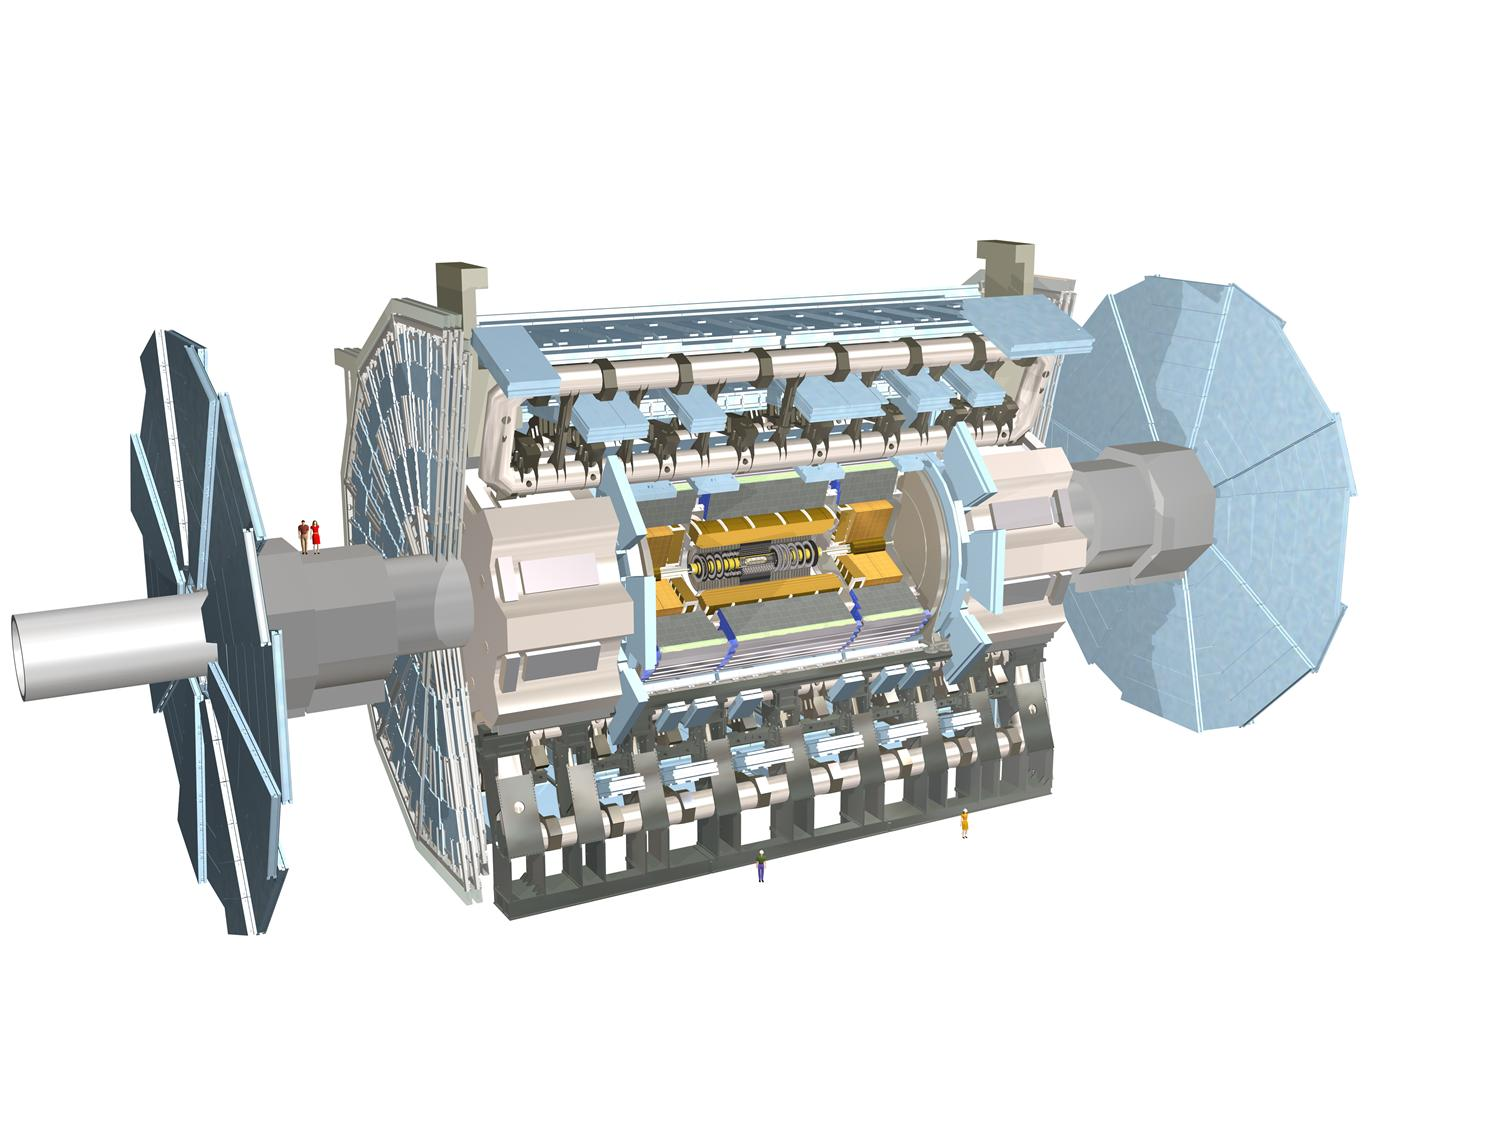
\includegraphics[width=.7\textwidth]{Images/intro/ATLAS_detector.jpg}
    \captionsetup{width=.8\linewidth}
    \caption{Overview of the ATLAS detector. From \cite{atlasDetectorTechnology}}
    \label{fig:ATLAS}
\end{figure}
